\chapter{Background}

\section{The \Beluga Language}

\section{The Implementation of \Beluga} \label{section:beluga-implementation}

This section presents an overview of the implementation of \Beluga before any contribution detailed in this thesis were made\footnote{Revision \href{https://github.com/Beluga-lang/Beluga/tree/3db1ffd08d4c3bde7ad2ceb924bfb95488eef2b2}{3db1ffd08d4c3bde7ad2ceb924bfb95488eef2b2} on Github.}.

\Beluga is implemented following the pipeline architectural pattern, whereby processing of a \Beluga signature is implemented in distinct phases, and data flows in a feed-forward fashion throughout.
The compilation of \Beluga programs to machine code is not supported, so the implementation only covers the frontend component of compilation, which is responsible for parsing and semantic analysis of programs.
Since \Beluga is a dependently-typed language featuring code coverage analysis and termination checking, this semantic analysis process is complex.

\begin{figure}
\centering
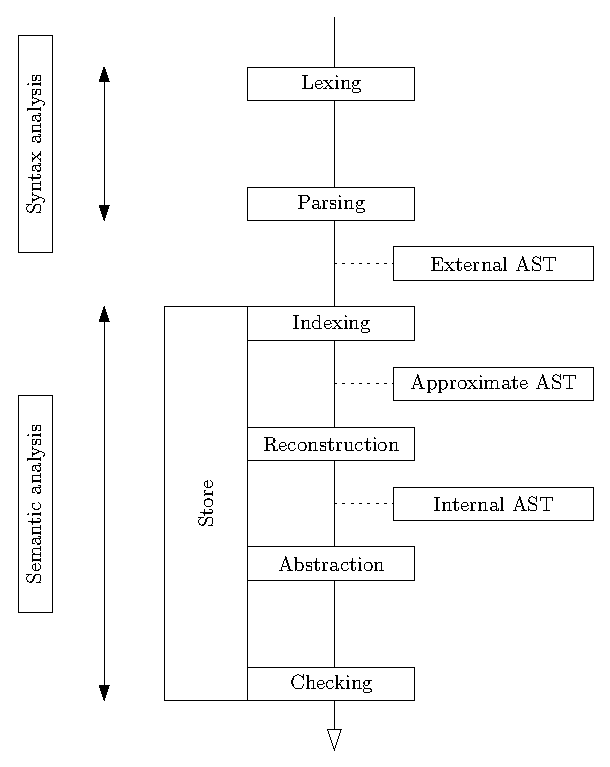
\includegraphics{figures/legacy-beluga-processing-pipeline.eps}
\caption[Overview of the implementation of \Beluga version \texttt{1.0.0}'s processing pipeline.]{%
Overview of the implementation of \Beluga version \texttt{1.0.0}'s processing pipeline.
The syntax analysis process converts the textual representation of \Beluga programs into an initial \acs{AST}.
The semantic analysis process refines this \acs{AST} by performing type-directed signature reconstruction, using global mutable data structures that include a store of signature entries.
}
\label{figure:legacy-beluga-processing-pipeline}
\end{figure}

As illustrated in figure~\ref{figure:legacy-beluga-processing-pipeline}, the processing of a \Beluga signature starts with syntax analysis, which is comprised of a tokenization and parsing phase that converts the textual representation of the signature to an \ac{AST}, called the external \ac{AST}.
The model for this \ac{AST} contains ambiguous nodes, meaning that some \ac{AST} node variants capture multiple parse trees.
Specifically, the application of \LF type-level and term-level constants is represented as a list of parsemes.
Parsing of signature-level declarations also features mixing/unmixing flags (auxiliary data types for bookkeeping) to postpone some elements of disambiguation to phases after context-free parsing.

Indexing in \Beluga is the process where the concrete syntax is elaborated to an approximate syntax in which most variables are replaced with de Bruijn indices.
This process is run after parsing, and is also responsible for disambiguating the juxtaposition of \LF parsemes at the precedence level of applications (which may contain user-defined operators), as well as disambiguating \LF types from terms and resolving constants.
This design is sensible since computing de Bruijn indices requires a stateful traversal of the \ac{AST} that accumulates lists of bindings to produce the referencing environment.
Using the centralized store of declarations, some measure of overloading of identifiers is supported using a pre-defined order of lookups in the referencing environment based on the kind of identifier that is expected for a given \ac{AST} node.
For instance, computation-level identifiers are resolved by looking up in order the store of computation-level variables, the store of program constants, and then the store of data type constructors.
Since names appearing in the \LF level are not part of this name resolution strategy, then an identifier can be overloaded to stand for an \LF term as well as a computation-level expression.

After indexing, the reconstruction~\cite{pientka2013insider} phase is run to reconstruct holes in types and terms, both at the \LF level and the computation level.
These holes stand for arguments omitted by the user, and provide an elegant way of abbreviating otherwise tedious aspects of programming with dependent types.
At the \LF level, approximate types are constructed to partially check the kinding of \LF types and the typing of \LF terms, as well as for guiding the synthesis of normal terms that check against a given type using typing constraints.
Type-driven unmixing of overloaded syntactic forms occurs at the meta-level, whereby meta-objects are disambiguated from substitutions during reconstruction.
The approximate \ac{AST} provides a disambiguated representation of the overall \Beluga signatures, which helps in keeping track of the various changes made during this complicated phase.

A nearly complete internal \ac{AST} is produced at the end of reconstruction.
An abstraction phase is run to abstract over free variables, which effectively introduces binders for implicit parameters.
% TODO: Expand

Finally, a semantic checking phase is run to ensure signature reconstruction and abstraction yielded valid programs.
This includes performing type-checking, coverage-checking and totality-checking.
These processes guarantee, respectively, that \LF-level and computation-level expressions are well-typed, that case analyses are exhaustive, and that functions annotated with a totality declaration terminate for all inputs.
% TODO: Expand

Starting with the indexing phase, data is shared between the phases of signature reconstruction using a global mutable store.
This auxiliary data structure is a set of tables mapping constant identifiers to meta-data like in a relational database.
Crucially, the referencing environment used during indexing is computed using this store.
% TODO: Expand

% TODO: Interactive REPL and Harpoon

% TODO: What the focus of this thesis is

\section{Stateful and Incremental Program Development}

Incremental program development in compiler design is the problem of applying edit actions to programs in \ac{AST} or representation while only re-processing a minimal portion of the program under edit.

% What is the key problem in incremental program development?
One of the main challenges in implementing incremental program development is that a compilation unit may only be revisited with the processing state it was defined in.
This means, for instance, that a process performing name lookups or mutations on the \ac{AST} at a given node may only do so using the variables and declarations in scope at that \ac{AST} node, just as the user does when editing the textual representation of that \ac{AST} node.
As such, edit actions on an \ac{AST} must preserve its semantic correctness properties so that serializing and subsequently deserializing it produces the same \ac{AST}.
This problem arises when a compiler is extended to support user interactions or non-sequential compilation steps.

% What are some user interactions that need to be scope safe?
In the context of tooling for a programming language, users benefit from interacting with the code they are editing by way of auxiliary software that performs actions on the textual representation of the program or its \ac{AST}.
These actions range widely in functionalities depending on the programming language's features, but typically include automated code formatters, linters, debuggers, type inspectors, code-completion suggestions, as well as edit actions to assist in refactoring existing code.
These tools are typically implemented separately from the compiler, and hence may only be reliably implemented with respect to a specification of the language.

% TODO: Figure of a DAG

% What are some non-sequential compilation steps that need to be scope safe?
Non-sequential processes in compiler design refer to compilation steps that occur concurrently, or occur using a subset of the data from previous compilation phases.
In general programming languages, these processes typically appear in the incremental compilation of programs whose dependency relation on compilation units may be arranged in a lattice.
To implement this, a \ac{DAG} of the compilation units is constructed where edges denote dependency.
A topological ordering is then computed for that \ac{DAG}, and used to create a compilation schedule with forked compilation processes for independent compilation units.
This enables parallelism to be used to reduce compilation time, and potentially the number of compilation units that need to be recompiled after an edit action is performed.
Implementing these features may require caching of compilation results and restoring processing states from those caches, which naturally raises the concern of cache invalidation.
Indeed, an incremental compilation process needs to be resumed in the state it originally happened, and changes that occur as a result of this compilation need to be propagated to the rest of the compiler's state.
This in turn triggers additional compilation steps for units that have explicit or transitive dependencies on the newly compiled unit.

% What is the general solution to the name resolution problem in incremental program development?
The general solution to stateful and incremental program development is to parameterize the non-sequential compilation processes with a visiting state that can be built in parallel with other processes.
For instance, a visiting state can be defined on a named \ac{AST} to recompute the referencing environment up to the point where a new node needs to be processed and spliced in so that name resolution can be resumed from that point.
The issue then becomes how to efficiently construct and preserve the correctness of such visiting states, specifically in compilers for functional programming languages like \Beluga, and \acp{REPL} instantiated at program holes.

% An open stateful function is a function parameterized over some state, and the lifecycle of the mutable state is extrinsinc.
% A closed stateful function is a function that internally uses mutable states, whose lifecycle is intrinsically maintained.
